\chapter{NDVI-MAP FUNCTIONS AND USER GUIDE}
\label{chap:ndvi & it's user guide}

\section{What can app do?}

Application enables the user to envision \gls{ndvi} mean information stored in the database. It likewise gives the usefulness of sending out the information into \gls{csv} record and messaging it to anyone that needs it. This causes the user to visualize information utilizing diverse levels such as Country, State and Eco-District wise.

\section{A user guide/manual}

A guide is a short reference to some particular aspects of a software product. The user guide of the application is explained below.

\begin{itemize}
    \item \textbf{Downloading the app} \\
    At the presen time, the app is in process of being submitted to App Store for review. Once it is approved by Apple, anyone can utilize the "EyesOnCrops" application by downloading it from the Apple Store. 
    
    \begin{itemize}
        \item Open the App Store and type "EyesOnCrops" in search bar.
        \item Download and introduce the "EyesOnCrops" application on the device.
        \item Once installed, it will look like Figure~\ref{fig:app_icon_screen}.
        
        \begin{figure}[H]
            \centering
            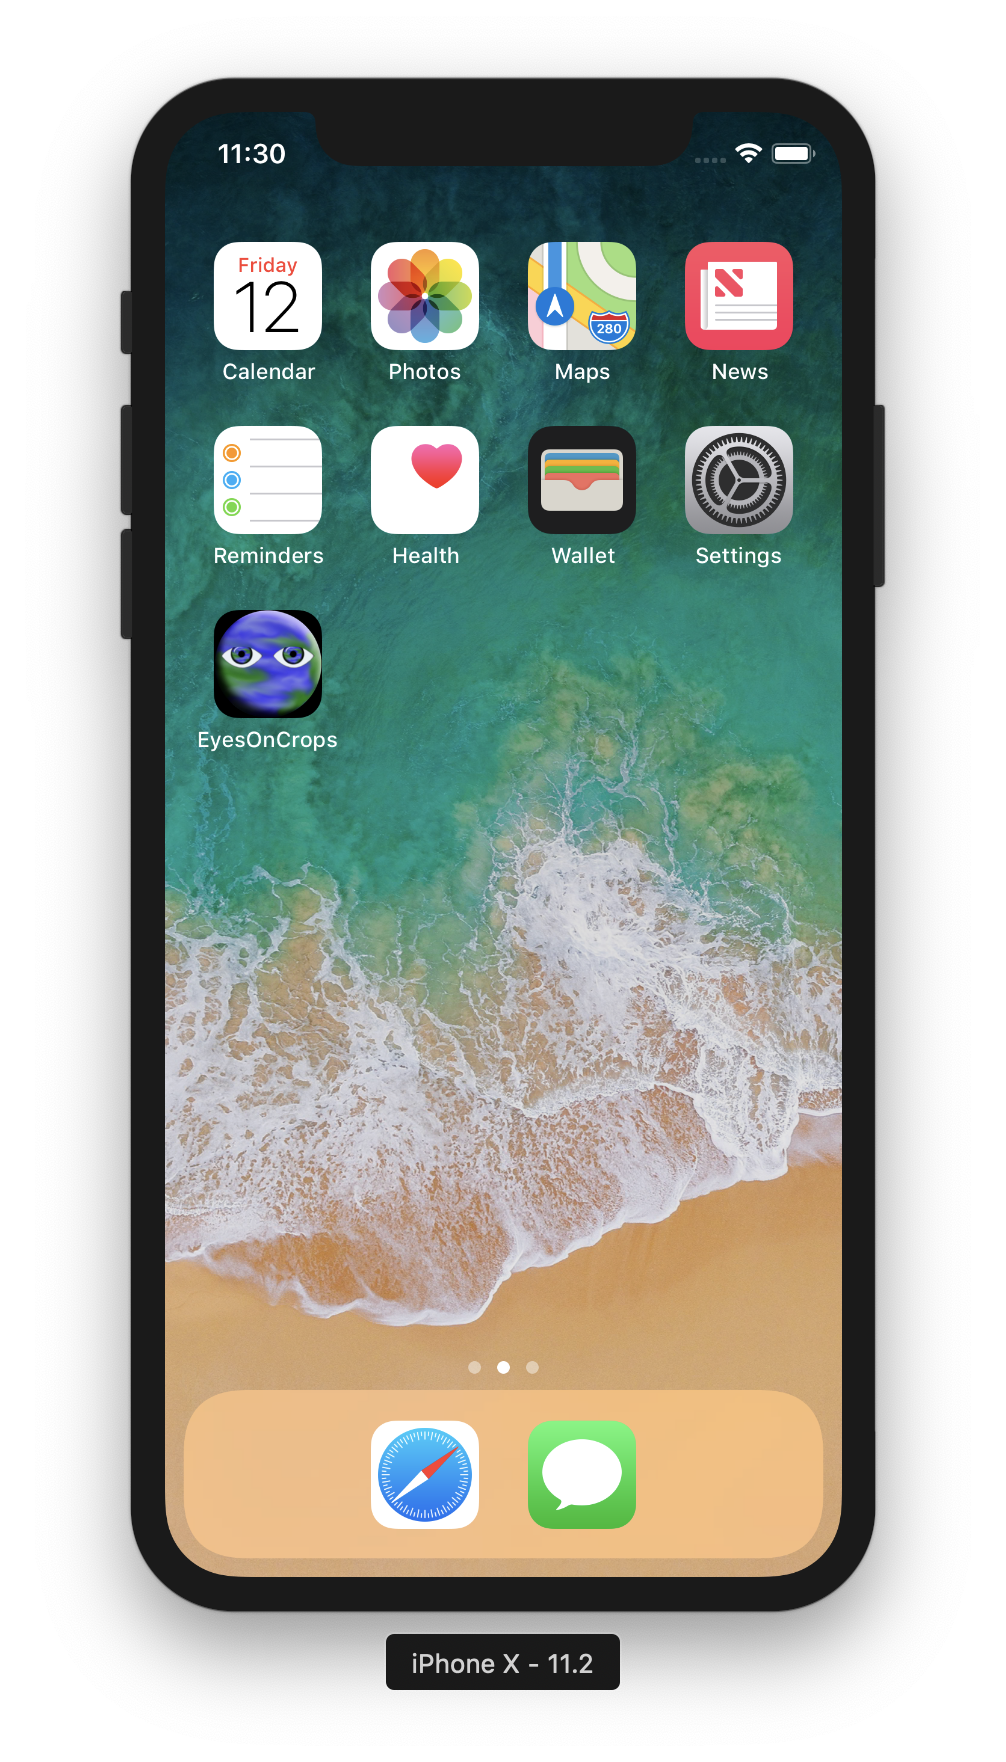
\includegraphics[width=0.50\linewidth]{figures/ch2/app_icon_screen.png}
            \caption{\label{fig:app_icon_screen} iPhone screen after downloading the app}
        \end{figure}
    \end{itemize}
    
    \item \textbf{Getting in the app} \\
    By tapping on app icon on Figure~\ref{fig:app_icon_screen}, it will lake the user to landing screen of the app, also known as the main screen. This screen gives two options, which are shown in Figure 2.2.
     
        \begin{figure}[H]
            \centering
            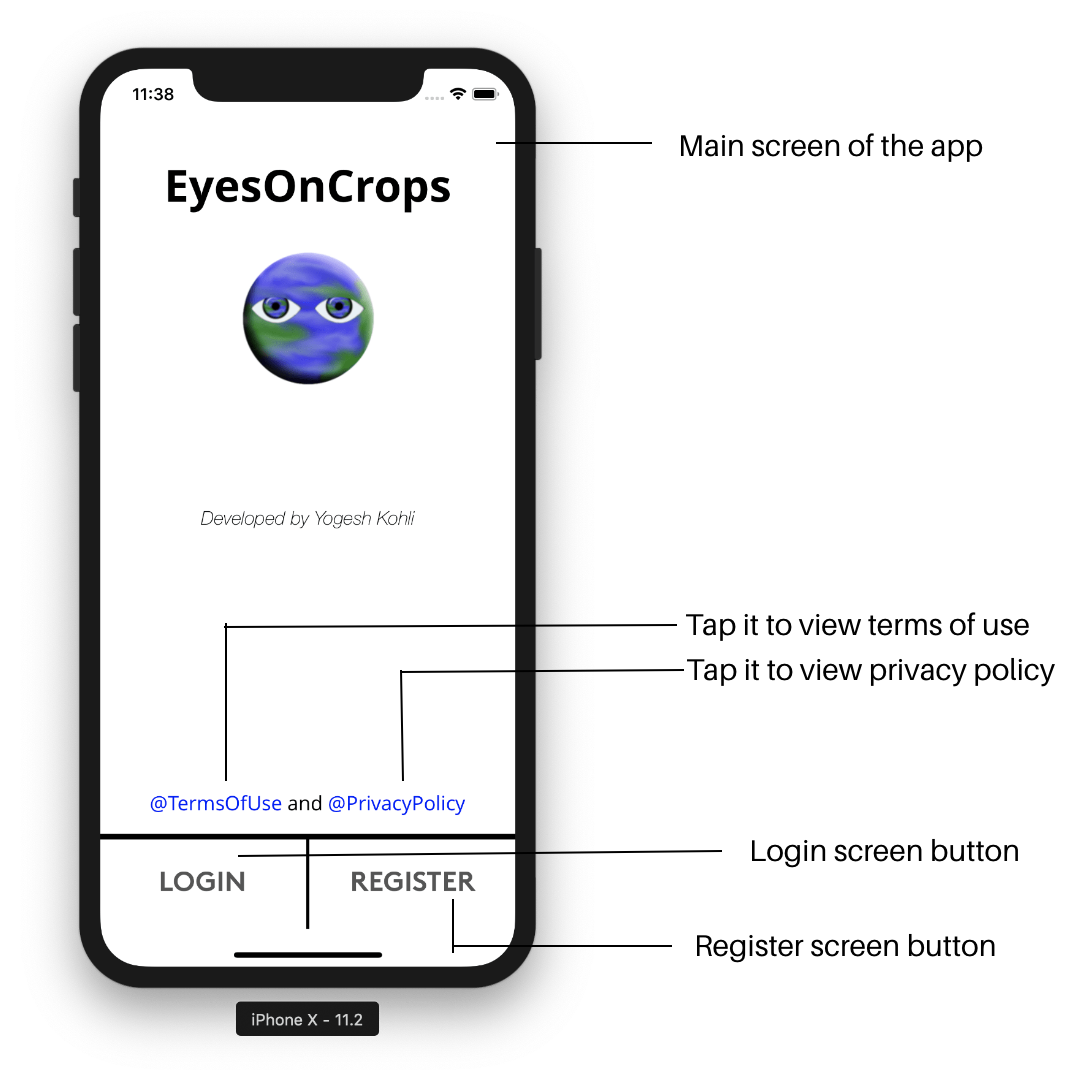
\includegraphics[width=0.50\linewidth]{figures/ch2/main_screen.png}
            \caption{\label{fig:main_screen} Main / Landing screen of the app}
        \end{figure}

    \textbf{1. Register} \\
    \textbf{2. Login} \\
    
    By selecting "\textbf{Register}" in Figure~\ref{fig:main_screen}, the user is taken to registration process. This is divided into 5 steps which are explained below.
    
        \begin{figure}[H]
            \centering
            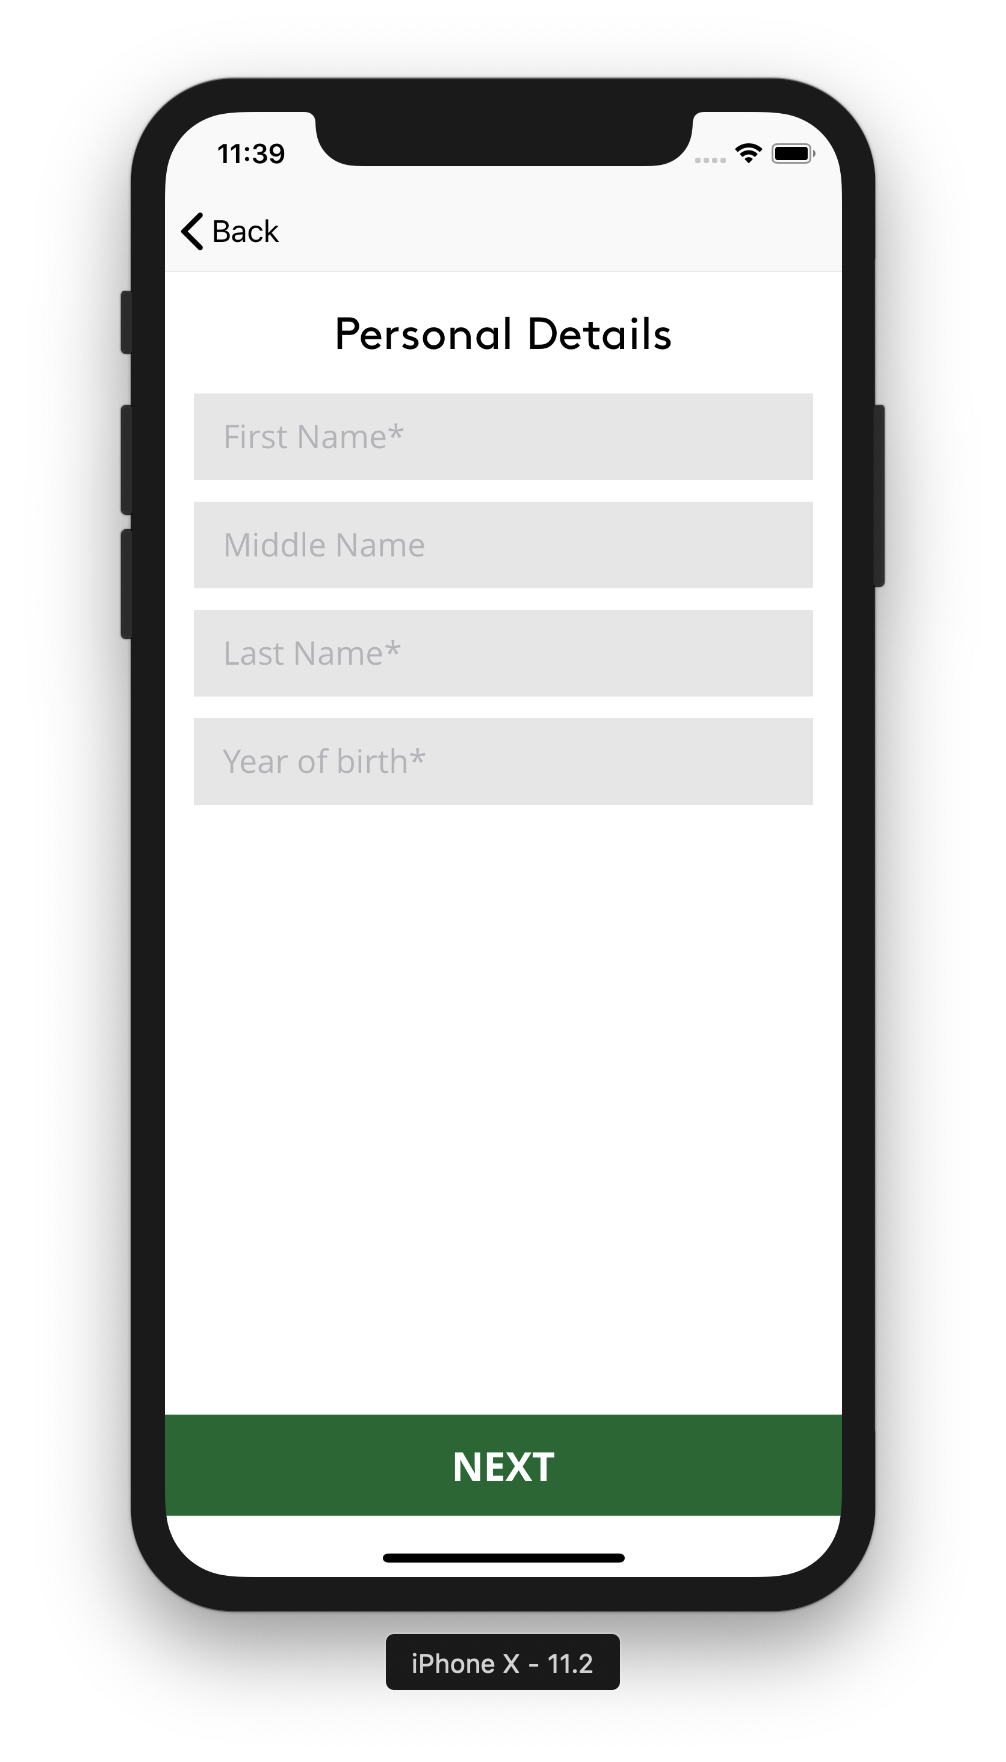
\includegraphics[width=0.50\linewidth]{figures/ch2/register_personal.png}
            \caption{\label{fig:register_personal} Personal details screen - Register process}
        \end{figure}
  
        
        \begin{figure}[H]
            \centering
            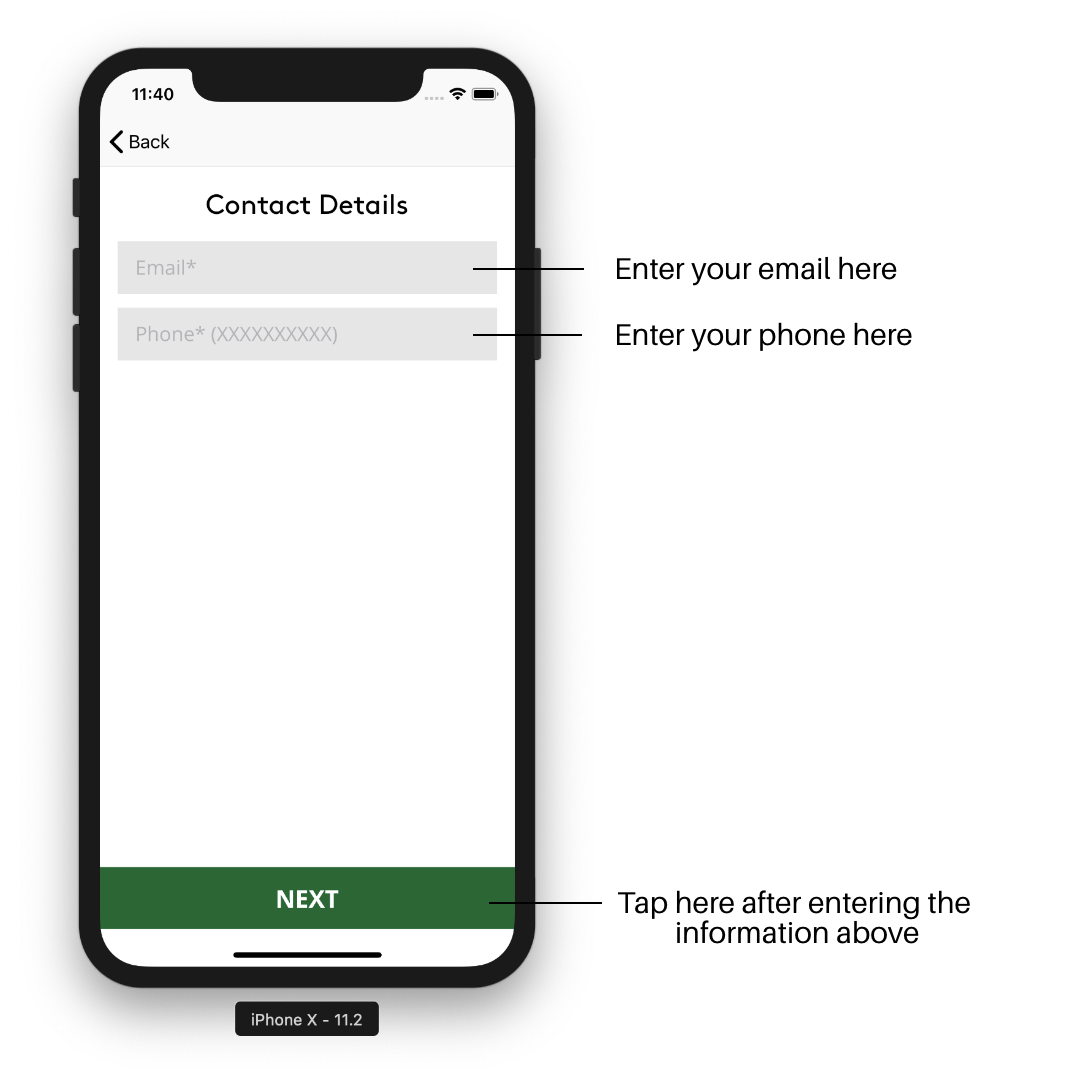
\includegraphics[width=0.50\linewidth]{figures/ch2/register_contact.png}
            \caption{\label{fig:register_contact} Contact details screen - Register process}
        \end{figure}
     
        \begin{figure}[H]
            \centering
            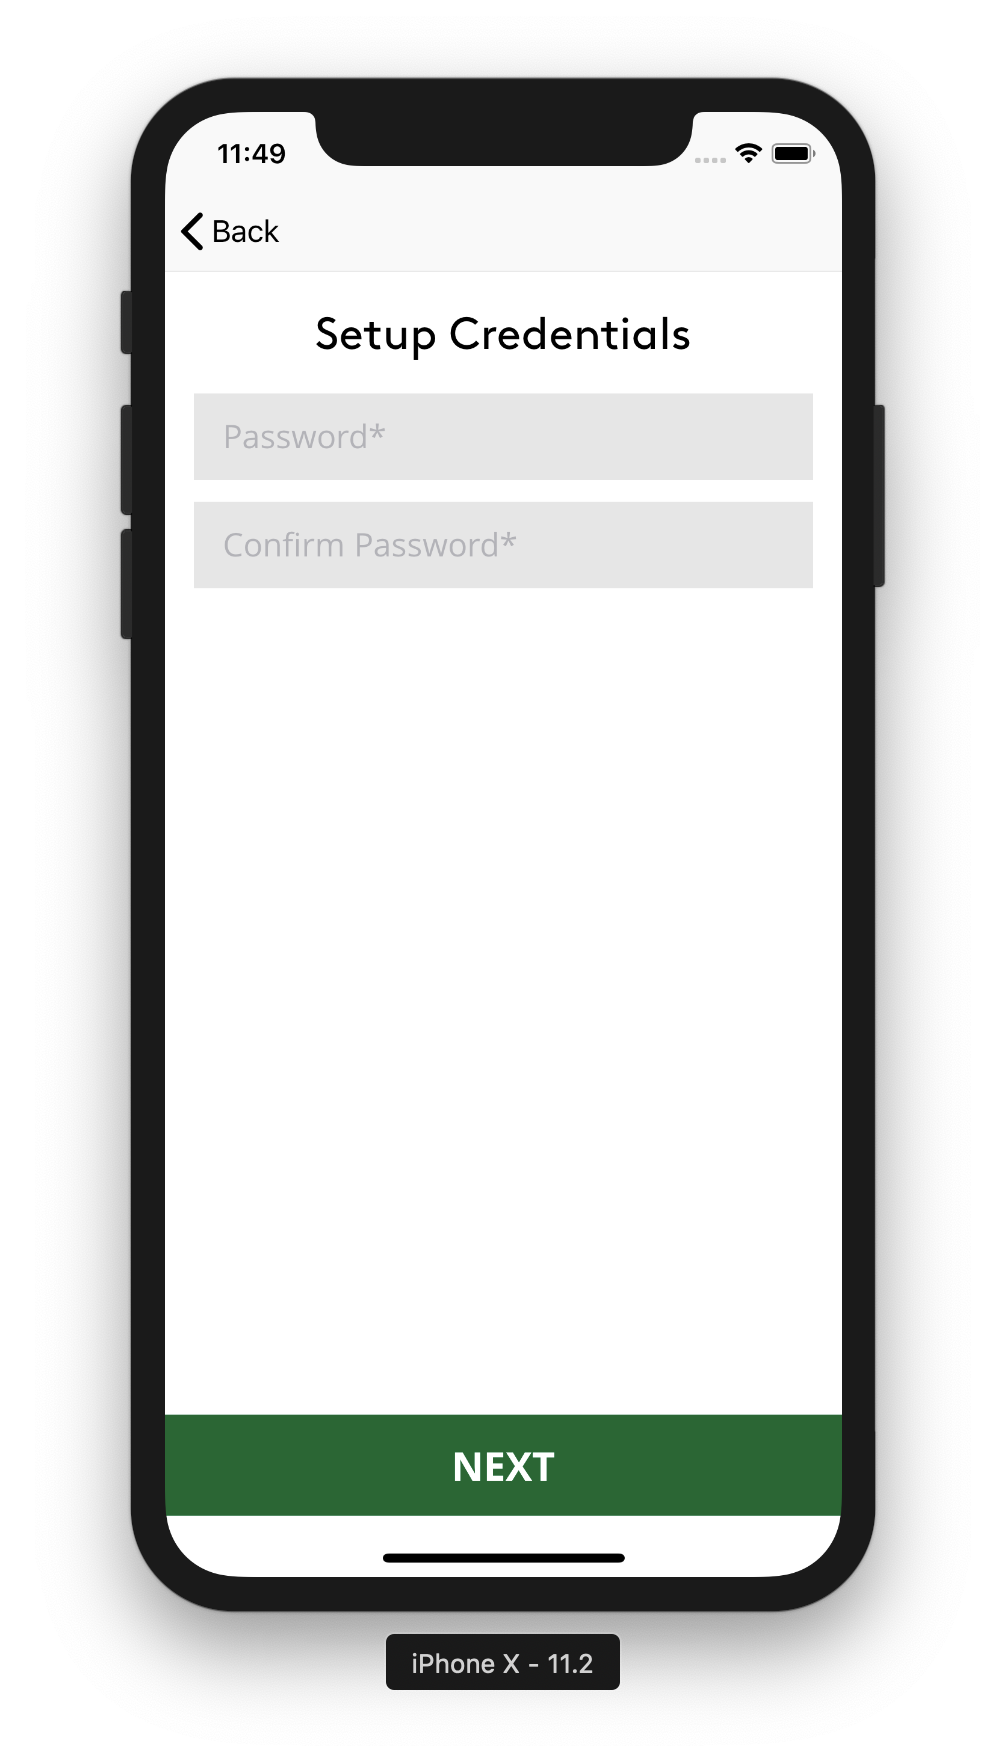
\includegraphics[width=0.50\linewidth]{figures/ch2/credentials_setup.png}
            \caption{\label{fig:credentials_setup} Setup credentials screen - Register process}
        \end{figure}
       
        
        \begin{figure}[H]
            \centering
            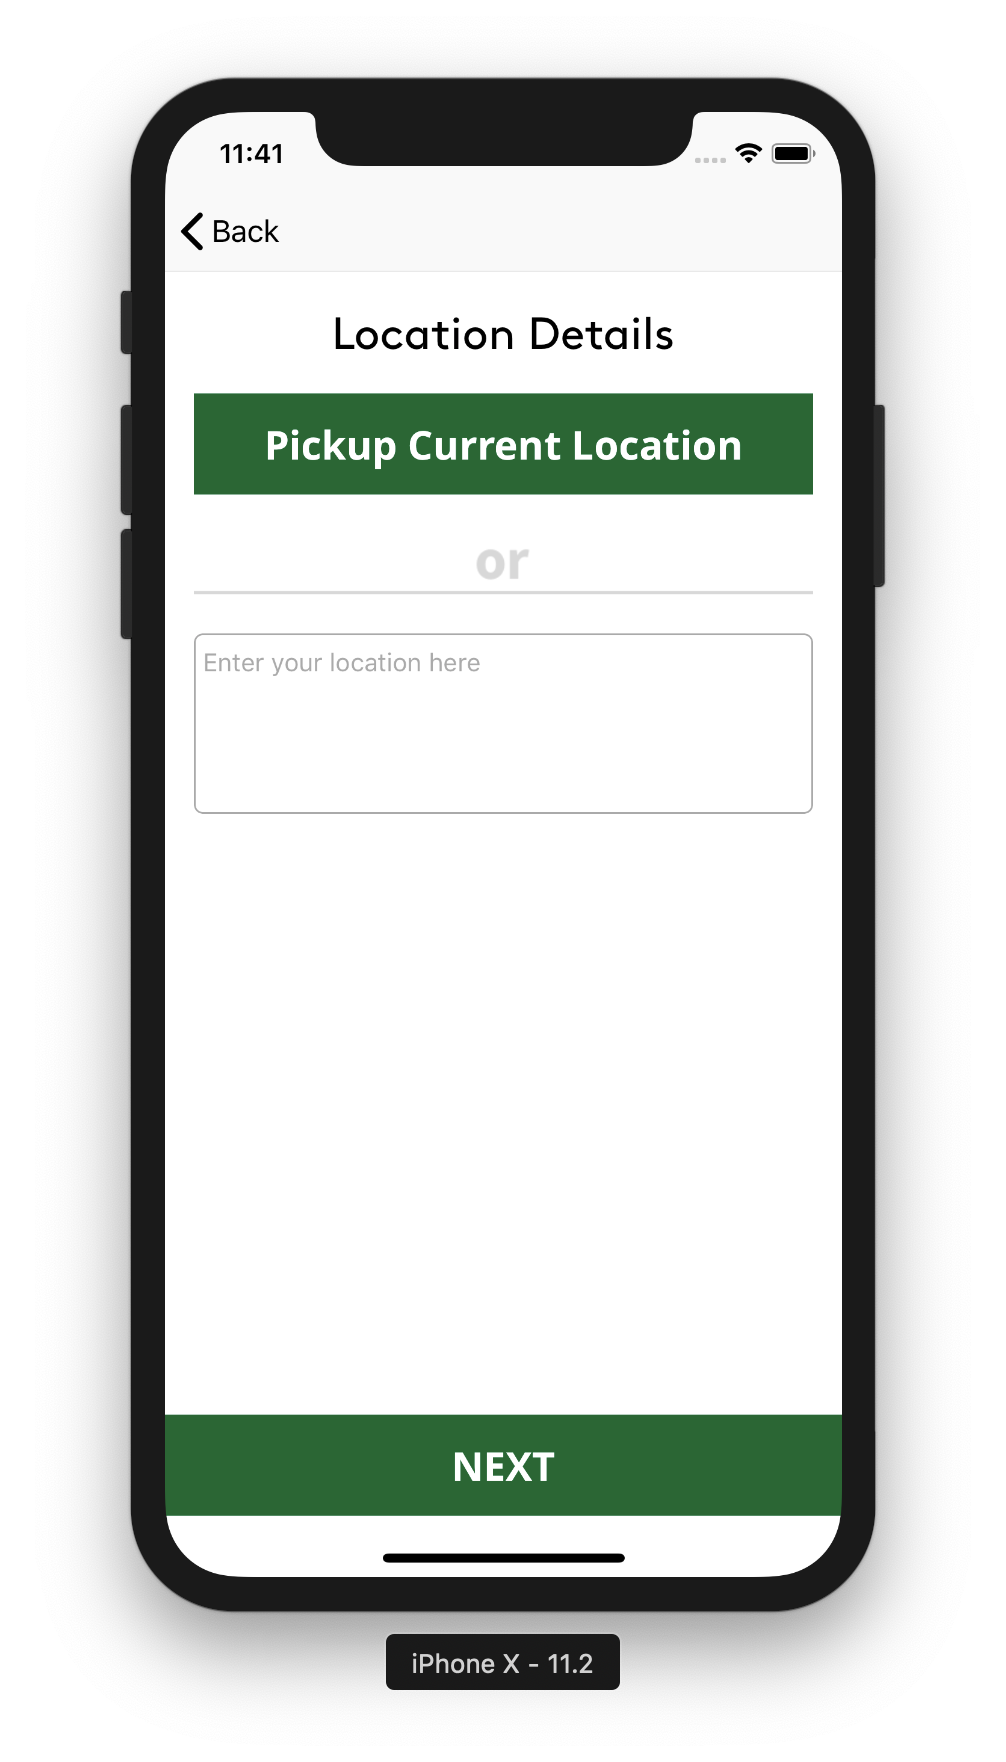
\includegraphics[width=0.50\linewidth]{figures/ch2/register_location.png}
            \caption{\label{fig:register_location} Location details screen - Register process}
        \end{figure}
 
        \begin{figure}[H]
            \centering
            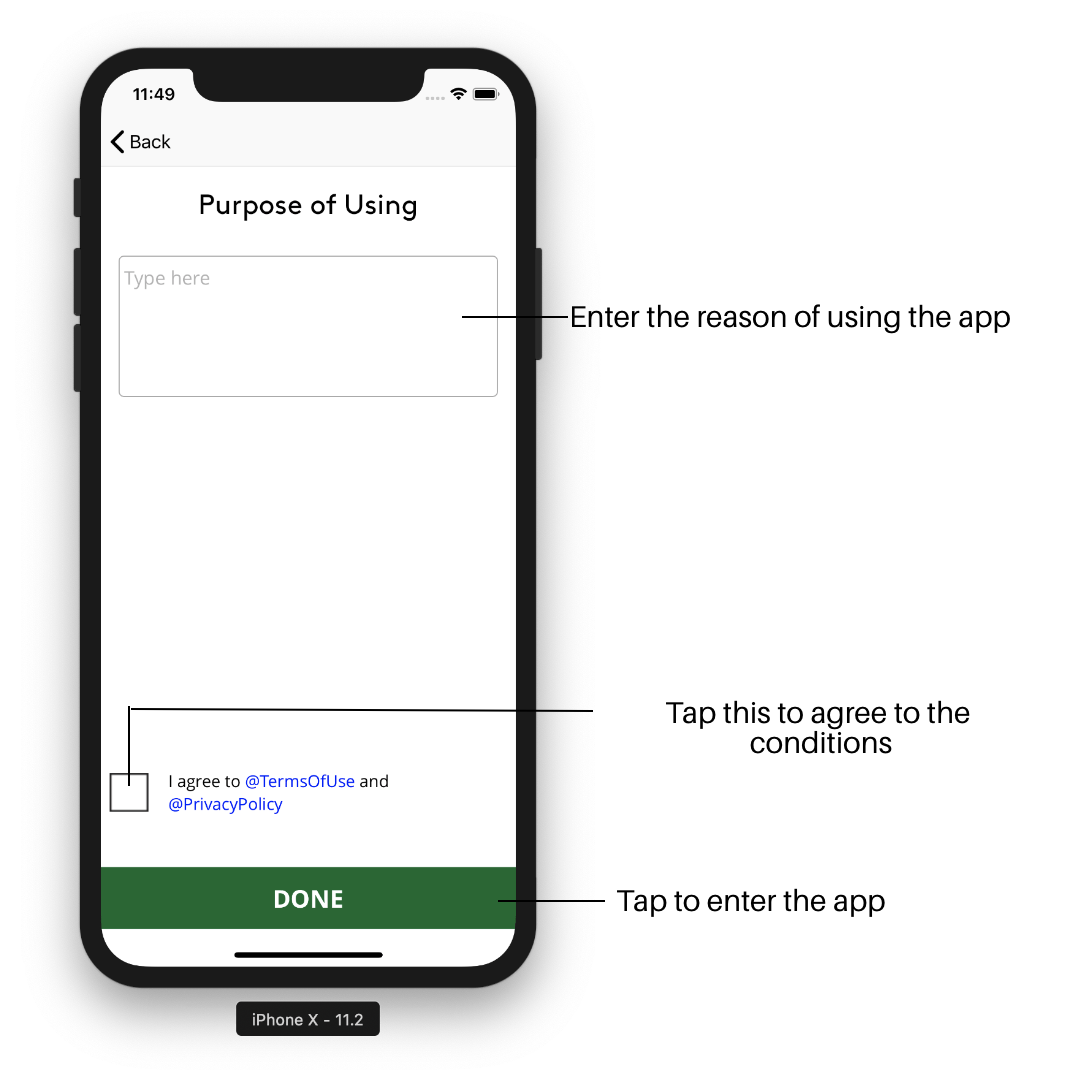
\includegraphics[width=0.50\linewidth]{figures/ch2/purpose_app.png}
            \caption{\label{fig:purpose_app} Purpose of using the app screen - Register process}
        \end{figure}

    
    By selecting "\textbf{Login}" in Figure~\ref{fig:main_screen}, the user is taken to the screen that gives options to enter the application which is shown in Figure~\ref{fig:loginOptions}.
    
    \begin{figure}[H]
            \centering
            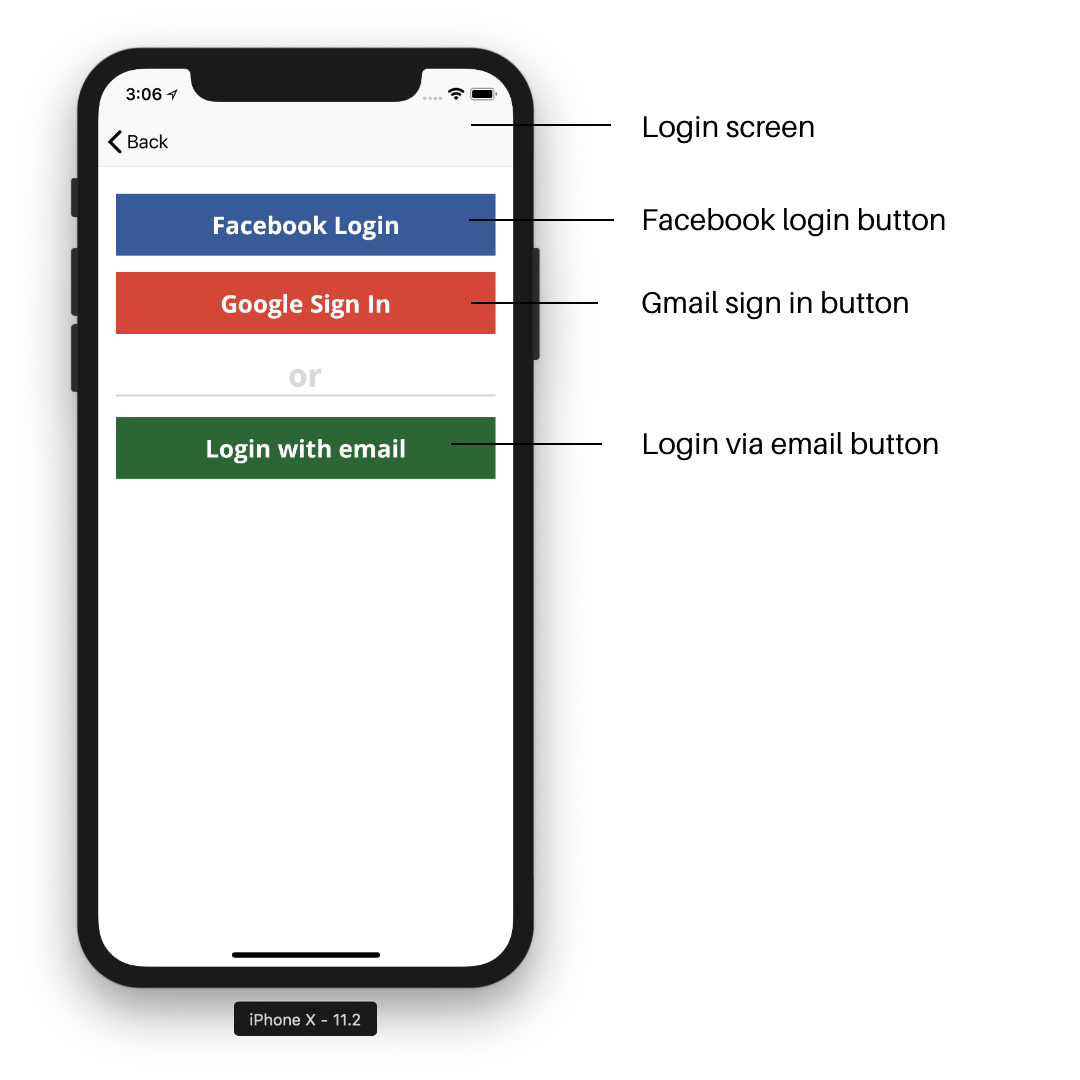
\includegraphics[width=0.50\linewidth]{figures/ch2/loginOptions.png}
            \caption{\label{fig:loginOptions} Login options in the app}
    \end{figure}
    
     \textbf{1. Login via Social Accounts}
     \begin{itemize}
         \item Facebook login
         \item Gmail login
     \end{itemize}
   
     \textbf{2. Login via Email} \\
    This screen requires the user credentials to enter the application. The screen has appeared in Figure~\ref{fig:login_email}.
     
     \begin{figure}[H]
            \centering
            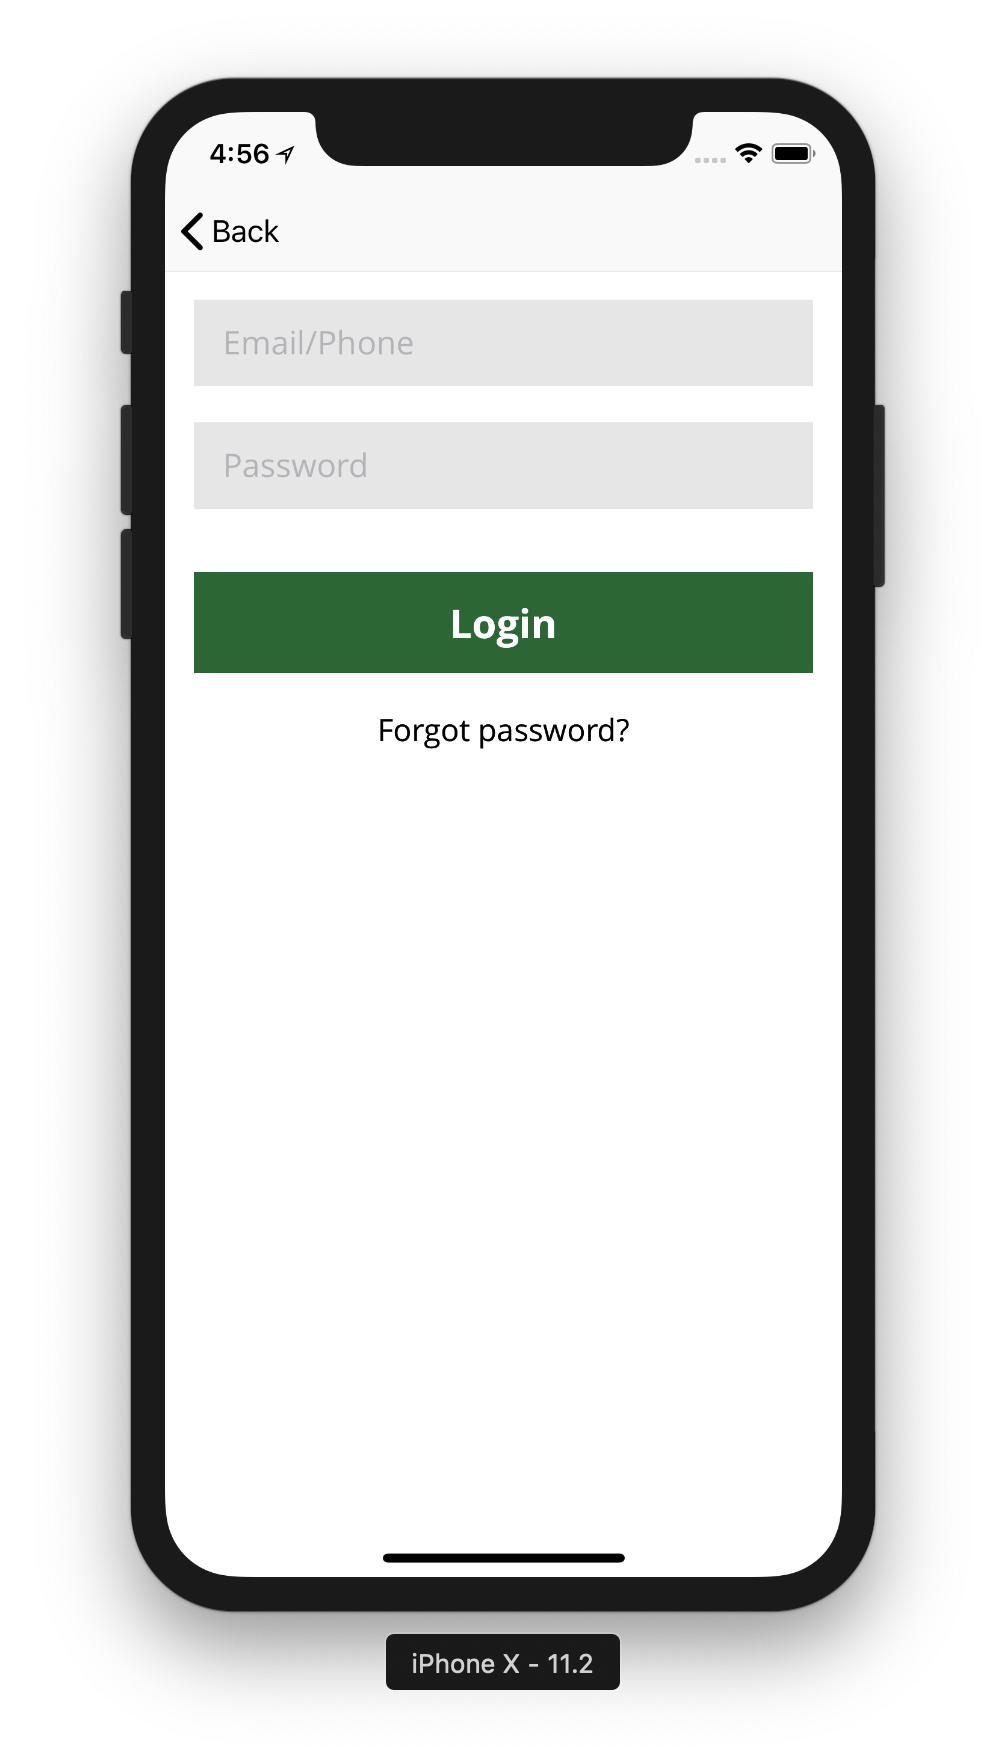
\includegraphics[width=0.50\linewidth]{figures/ch2/login_email.png}
            \caption{\label{fig:login_email} Login via email}
    \end{figure}
    
    
    \item \textbf{Home} \\
    By login in the application, the user arrives to the home screen which fundamentally has everything to use the application.
    
    \begin{figure}[H]
            \centering
            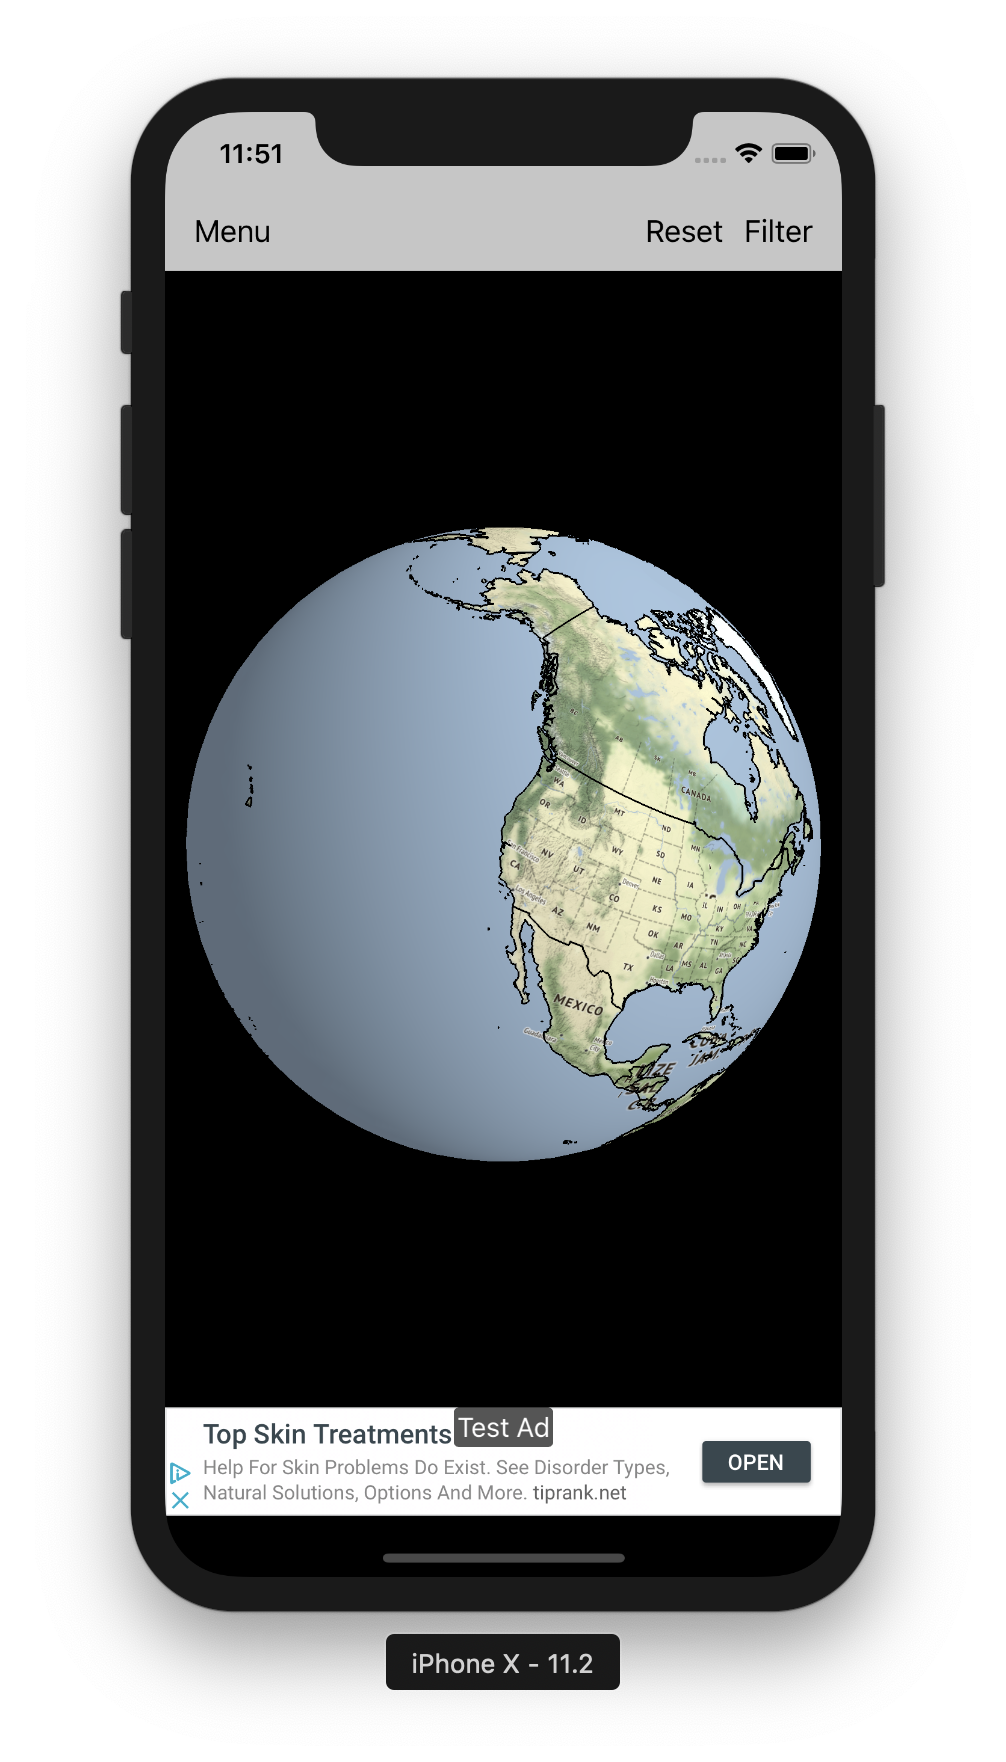
\includegraphics[width=0.5\linewidth]{figures/ch2/home.png}
            \caption{\label{fig:home_screen} Home page - landing page after login}
    \end{figure}
    

    \item \textbf{Slide out menu} \\
    Slide out menu has been utilized to give the application an extremely pleasant look in light of keeping the ease of use while exploring in the application. It has been shown in Figure~\ref{fig:side_menu}.
    
     \begin{figure}[H]
            \centering
            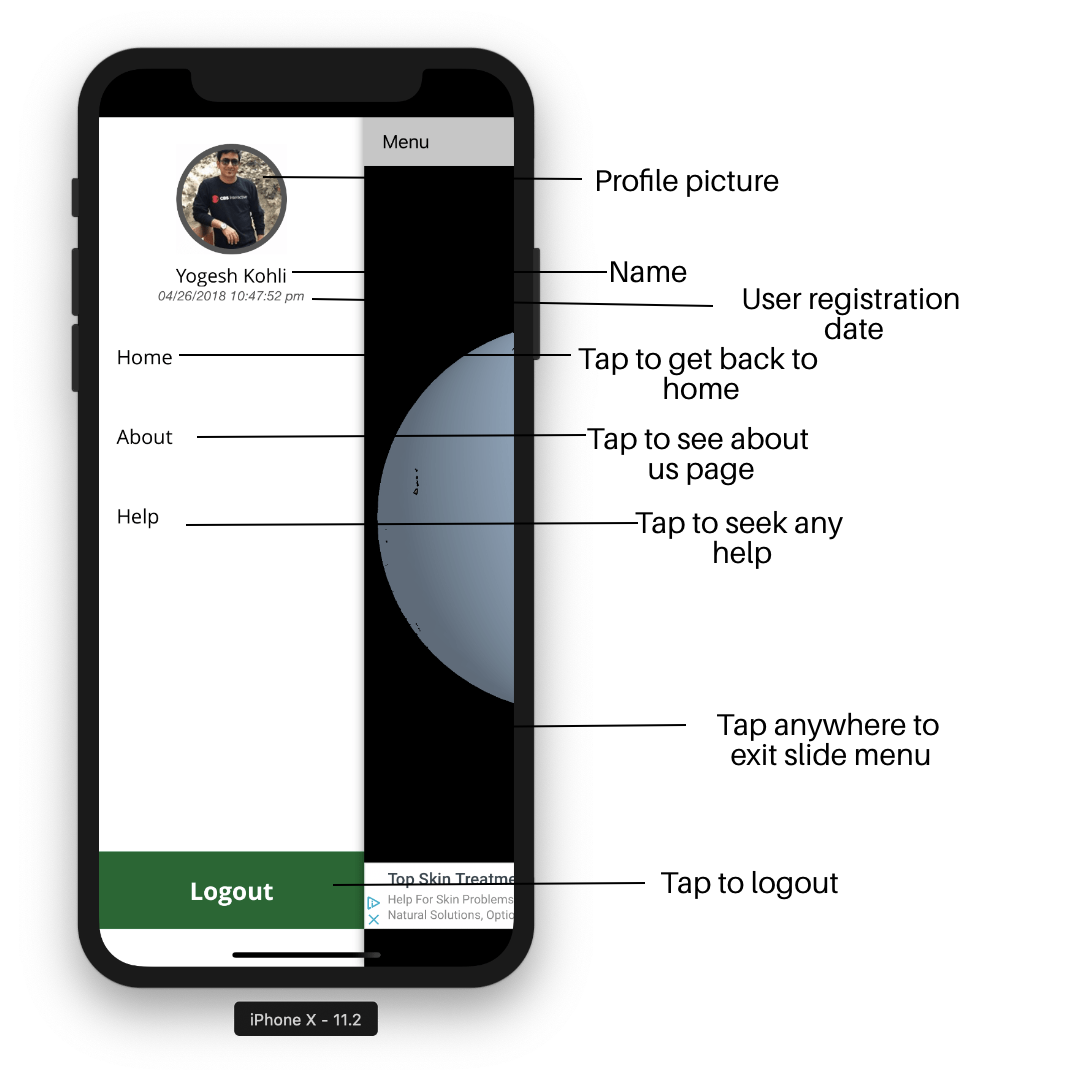
\includegraphics[width=0.50\linewidth]{figures/ch2/side_menu.png}
            \caption{\label{fig:side_menu} Slide out menu after selecting menu option on Home screen}
    \end{figure}
    
    
   \item \textbf{Filter screens} \\
    Tapping on filter button on home screen takes the user to Figure~\ref{fig:filter_screen}.
    
    \begin{figure}[H]
            \centering
            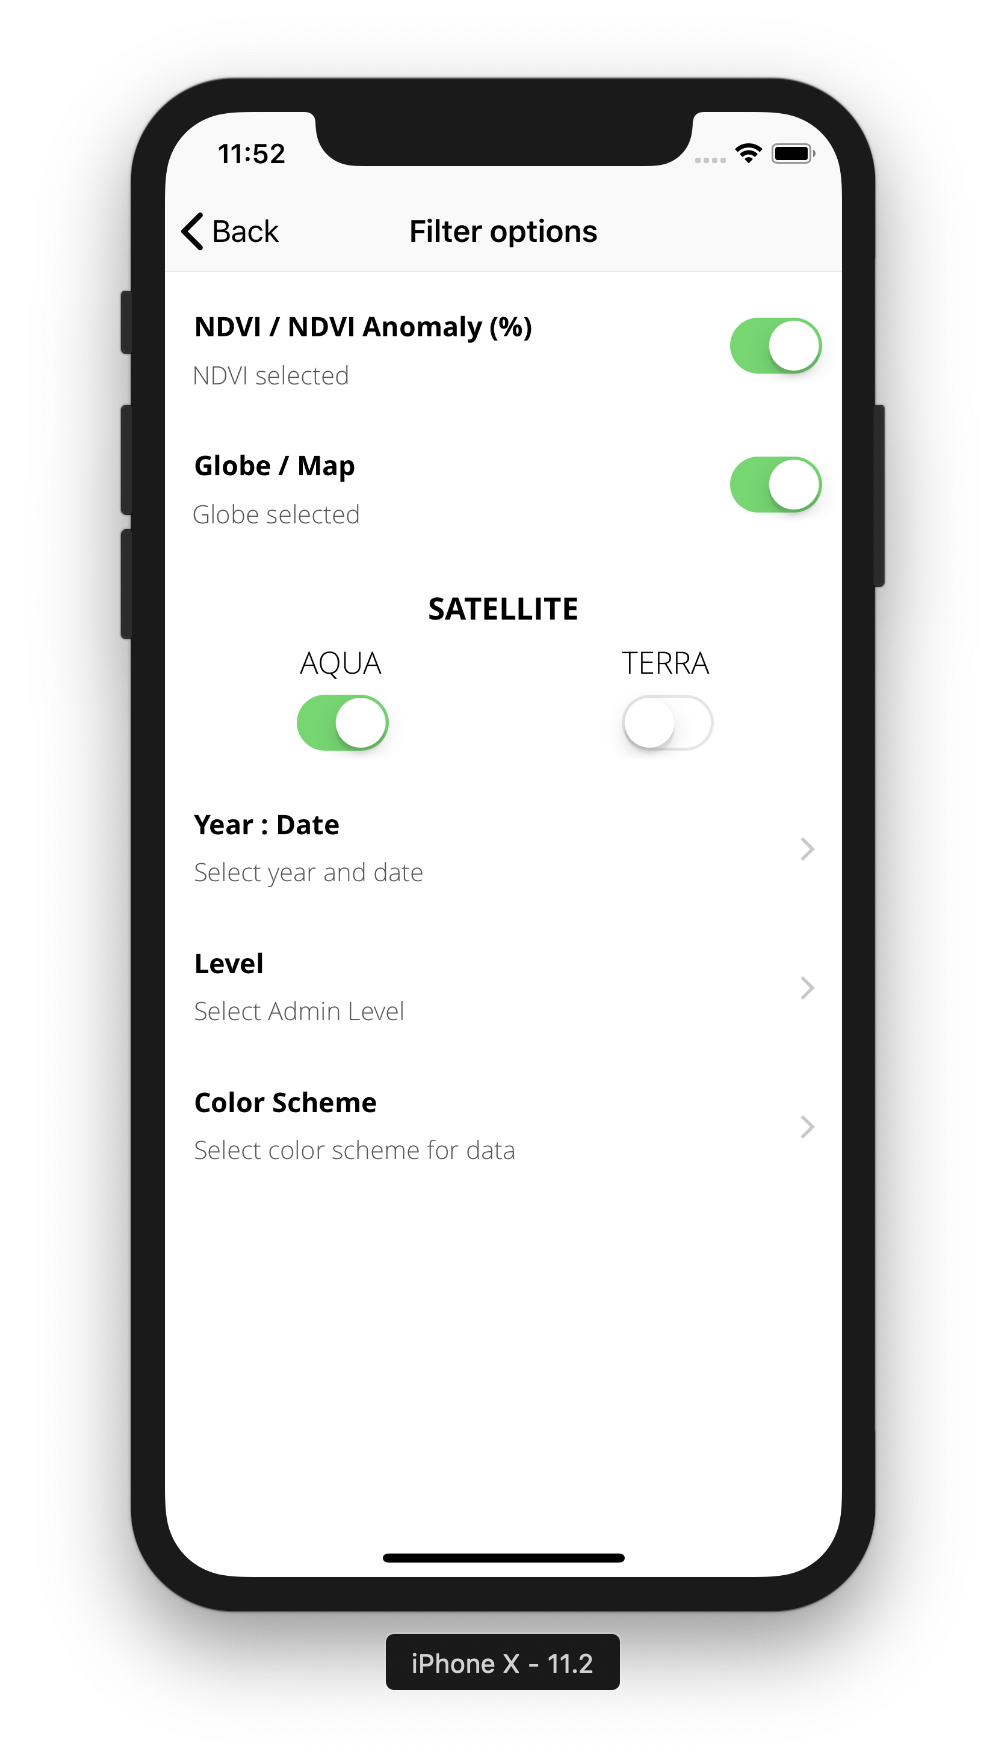
\includegraphics[width=0.50\linewidth]{figures/ch2/filter_screen.png}
            \caption{\label{fig:filter_screen} Filter screen after selecting filter option on Home screen}
    \end{figure}
    
    Now, there are various ways to filter the data which are mentioned below.
   
    \begin{itemize}
        \item \textbf{Year list}
        
        Year and Date wise selections on filter screen takes the user to the screen shown in Figure~\ref{fig:years_list_screen}.
        
         \begin{figure}[H]
            \centering
            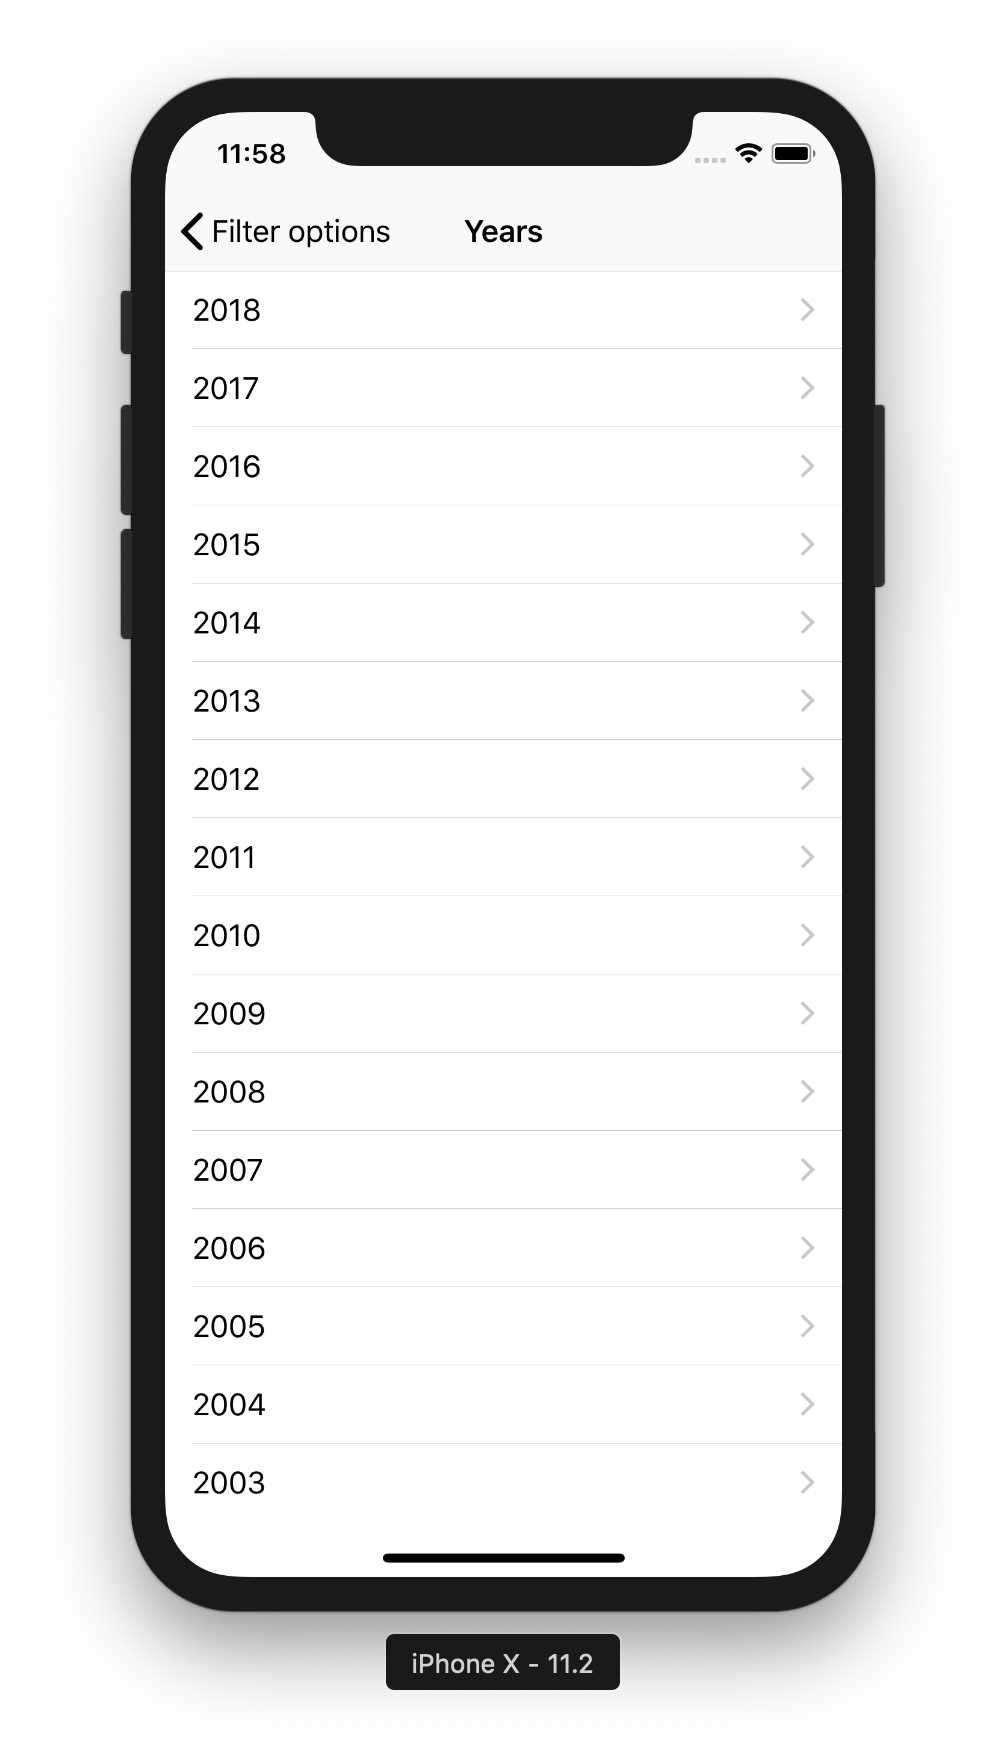
\includegraphics[width=0.50\linewidth]{figures/ch2/year_list.png}
            \caption{\label{fig:years_list_screen} Filter - Year list screen}
         \end{figure}
   
        \item \textbf{Admin level list}
        
        Admin Level tap takes the user to the screen shown in Figure~\ref{fig:level_list_screen}.
        
         \begin{figure}[H]
            \centering
            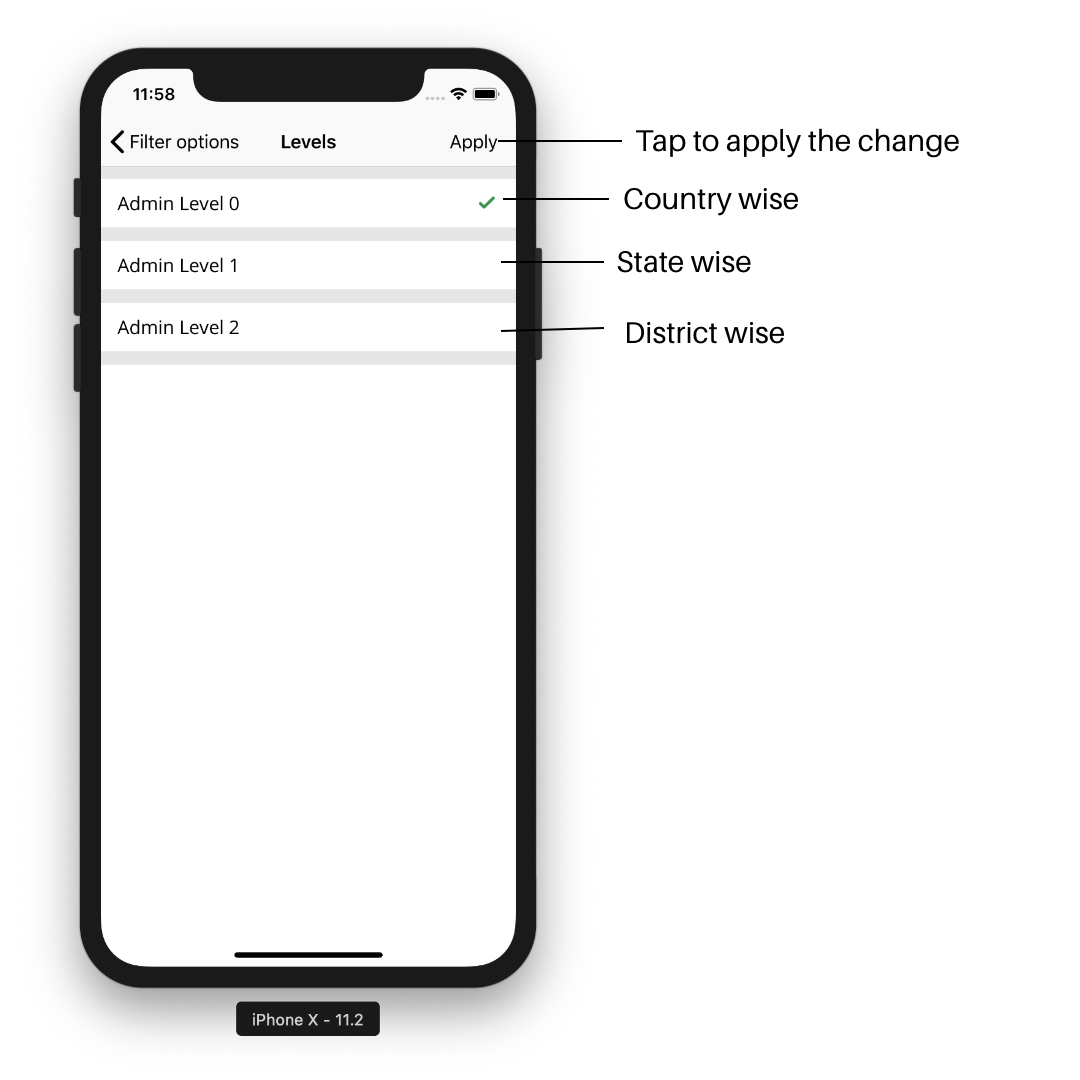
\includegraphics[width=0.50\linewidth]{figures/ch2/level_list.png}
            \caption{\label{fig:level_list_screen} Filter - Admin level list screen}
        \end{figure}

     \item \textbf{Color scheme list}
     
     Color scheme tap takes the user to the screen shown in Figure~\ref{fig:color_scheme}.
        
        \begin{figure}[H]
            \centering
            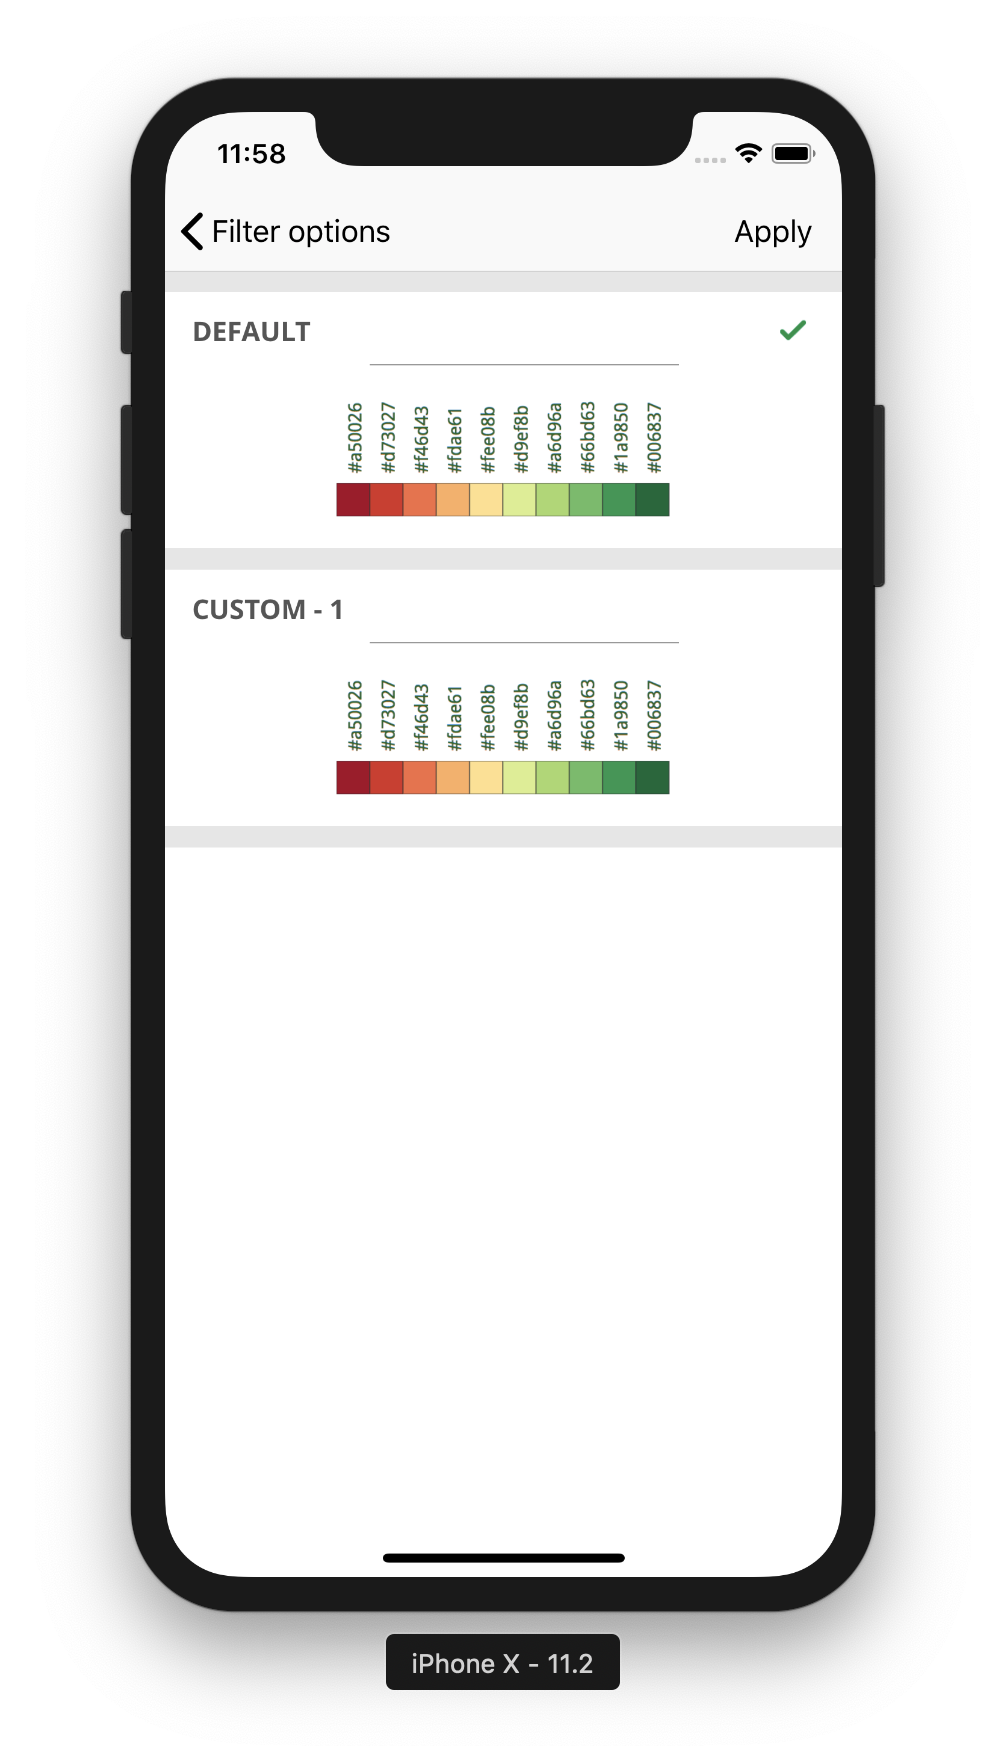
\includegraphics[width=0.50\linewidth]{figures/ch2/color_scheme.png}
            \caption{\label{fig:color_scheme} Filter - Color palette  options screen}
        \end{figure}
        
    \end{itemize}

\end{itemize}



